\documentclass{article}
\usepackage{amsmath}
\usepackage{amssymb}
\usepackage{graphicx}
\usepackage{hyperref}
\usepackage[version=4]{mhchem}

\title{Example 3}
\date{}

\begin{document}
\maketitle

(AMC) Figure \(A B C D\) is a trapezoid with \(A B / / D C ; A B=5\);\\
\(B C=3 \sqrt{2}, \angle B C D=45^{\circ}\) and \(\angle C D A=60^{\circ}\). The length of \(D C\) is

Solution: (D).\\
Drop perpendiculars from \(A\) and \(B\) to \(D C\), intersecting \(D C\) at \(F\) and \(E\), respectively. \(\triangle B E C\) is an isosceles right triangle, so \(B E=E C=3\). Since \(A B E F\) is a rectangle, \(F E=5\) and \(A F=3 . \triangle A F D\) is a \(30-60-90\) triangle, so \(D F\) \(=A F / \sqrt{3}=\sqrt{3}\).\\
\centering
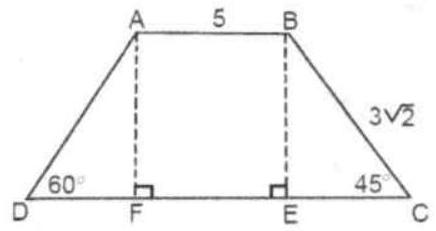
\includegraphics[width=\textwidth]{images/076(2).jpg}\\
\(D C=D F+F E+E C=\sqrt{3}+5+3=8+\sqrt{3}\).


\end{document}
